\section{Experiment}

Main goal: explain what you did with enough detail so the reader could reproduce it
Include the equipment used, quantities you measured (if relevant also the accuracy of the
equipment), procedures you followed
Diagrams (e.g. scheme of the circuit) can be included
Please do not include results here!




\subsection{Part 1}
During the first part of the lab we measured the intensity for a white diode with different voltages. The voltage was controlled through a DC-source shown in \autoref{fig:part1_circuit}. 






    
\subsection{Part 2}




\subsection{Part 3}




\begin{figure}[H]
    \centering
    \begin{subfigure}{0.3\textwidth}
        \centering
        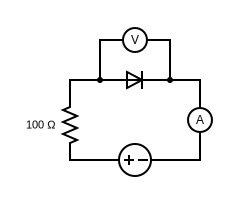
\includegraphics[width=\textwidth]{Figures/circuit_part1.png}
        \subcaption{This sktch shows the circuit for part 1 and part 2. }
        \label{fig:part1_circuit}
    \end{subfigure}
    \hspace{2cm}
    \begin{subfigure}{0.3\textwidth}
        \centering
        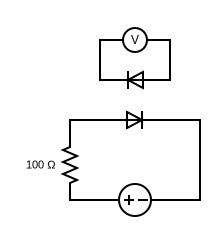
\includegraphics[width=\textwidth]{Figures/circuit_part3.png}
        \subcaption{This sktch shows the circuit for part 3, with the two different diodes. }
        \label{fig:part3_circuit}
    \end{subfigure}
    \caption{Above one can see the circuits used in this lab. Both circuits used an resistor with \SI{100}{\ohm}. }
    \label{fig:circuits}
\end{figure}
